\documentclass[a4paper,14pt]{extarticle}  % 14pt, 17pt, 20pt
% \documentclass[oneside,final,14pt]{extarticle} %
\usepackage[utf8]{inputenc}
\usepackage[T2A]{fontenc}
\usepackage[russian]{babel}
\usepackage{vmargin}
\usepackage{amsmath}
\usepackage[normalem]{ulem}
\usepackage{amssymb}
\usepackage{enumitem}
\usepackage[linesnumbered,ruled,vlined,titlenotnumbered]{algorithm2e}
% \setpapersize{A4}
% Шаблон для \setmarginsrb
%\setmarginsrb{leftmargin}{topmargin}{rightmargin}{bottommargin}%
%             {headheight}{headsep}{footheight}{footskip}
\setmarginsrb{30mm}{20mm}{15mm}{20mm}{0pt}{0mm}{0pt}{13mm}
\usepackage{indentfirst}
\usepackage{wrapfig}  % Для обтекания текста
\usepackage{graphicx} % Для вставки .jpg изображений
\usepackage{bbold}   % Для индикаторной функции
\usepackage{listings} % Для вставка кода в текст
\usepackage{setspace} % Для указание междустрочного интервала
\onehalfspacing       % Установка полуторного интервала

% Перевод плагина algorithm2e

\SetKwInput{KwData}{Исходные параметры}
\SetKwInput{KwResult}{Результат}
\SetKwInput{KwIn}{Входные данные}
\SetKwInput{KwOut}{Выходные данные}
\SetKwIF{If}{ElseIf}{Else}{если}{тогда}{иначе если}{иначе}{конец условия}
\SetKwFor{While}{до тех пор, пока}{выполнять}{конец цикла}
\SetKw{KwTo}{от}
\SetKw{KwRet}{возвратить}
\SetKw{Return}{возвратить}
\SetKwBlock{Begin}{начало блока}{конец блока}
\SetKwSwitch{Switch}{Case}{Other}{Проверить значение}{и выполнить}{вариант}{в противном случае}{конец варианта}{конец проверки значений}
\SetKwFor{For}{цикл}{выполнять}{конец цикла}
\SetKwFor{ForEach}{для каждого}{выполнять}{конец цикла}
\SetKwRepeat{Repeat}{повторять}{до тех пор, пока}
\SetAlgorithmName{Листинг}{лислинг}{Список алгоритмов}
\graphicspath{{./img/}}


\begin{document}
\begingroup
       \fontsize{12pt}{12pt}\selectfont

\begin{titlepage}
    \begin{center}
    МИНИСТЕРСТВО ОБРАЗОВАНИЯ И НАУКИ РОССИЙСКОЙ ФЕДЕРАЦИИ\\
    Федеральное государственное автономное образовательное учреждение\\
    высшего образования\\
    УРАЛЬСКИЙ ФЕДЕРАЛЬНЫЙ УНИВЕРСИТЕТ\\
    имени первого Президента России Б.\,Н.\,Ельцина\\
    \vspace{\baselineskip}
    ИНСТИТУТ ЕСТЕСТВЕННЫХ НАУК И МАТЕМАТИКИ\\
    \vskip +2cm
    Кафедра вычислительной математики и компьютерных наук\\
    \vspace{\baselineskip}
    \textbf{МНОГОМЕРНЫЙ АЛГОРИТМ ОВЫПУКЛЕНИЯ РОЯ ТОЧЕК, НАХОДЯЩИХСЯ В НЕОБЩЕМ ПОЛОЖЕНИИ}\\
    \vspace{\baselineskip}
    Направление \\09.04.03 «Прикладная информатика»\\
    \vskip +1cm
    \begin{tabular}{ l l }
    Допустить к защите: & Магистерская \\
    \hspace{3cm} & диссертация \\
    Зав. кафедрой: & \hspace{3cm}\\
     & \textbf{Корабельников}\\
    \hspace{3cm} & \textbf{Алексей Алексеевич}\\
    \hspace{3cm} & \hspace{3cm}\\
    \underline{\hspace{7cm}} & \underline{\hspace{7cm}}\\
    \hspace{3cm} & \hspace{3cm}\\
    Нормоконтролер: & Научный руководитель:\\
     & к.ф.-м.н. доц.  С. С. Кумков\\
    \hspace{3cm} & \hspace{3cm}\\
    \underline{\hspace{7cm}} & \underline{\hspace{7cm}}

    \end{tabular}

    \vfill

    Екатеринбург\\
    {2020}

    \end{center}
\end{titlepage}
\endgroup
\newpage
\setcounter{page}{1}
\thispagestyle{empty}

\section*{\centerline{РЕФЕРАТ}}

% \noindent
% \bigskip
% \noindent
Корабельников Алексей Алексеевич, «МНОГОМЕРНЫЙ АЛГОРИТМ ОВЫПУКЛЕНИЯРОЯ ТОЧЕК, НАХОДЯЩИХСЯ В НЕОБЩЕМ ПОЛОЖЕНИИ», работа содержит: стр. 22, рис. 3,
библ. 4 назв.


Ключевые слова: выпуклая оболочка, необщее положение точек, алгоритм.


Целью работы является разработка и реализация алгоритма построения выпуклой оболочки многомерного роя точек в случае их необщего положения. Под необщим положением точек подразумевается ситуация, когда в гиперплоскости $R^n$ измерения лежит больше чем $n+1$ точка. Наиболее перспективный с целью переноса в более высокую размерность оказался метод заворачивания подарка, поскольку он минимально использует специфику плоскости. В результате работы была разработана реализация алгоритма заворачивания подарка для работы в многомерном пространстве при необщем положении точек.

\newpage

\def\contentsname{\centerline{СОДЕРЖАНИЕ}}
\tableofcontents

\newpage
\section*{Введение}
\addcontentsline{toc}{section}{Введение}
Одна из фундаментальных проблем вычислительной геометрии является построение выпуклой оболочки конечного набора точек. На текущий момент, существует множество алгоритмов, решающих эту проблему. Эти алгоритмы широко применяются для решения задач в геометрическом моделировании, распознавании образов, экономике, статистики и в многом другом.

При работе алгоритмов может возникнуть проблема необщего положения точек. Если в гиперплоскости $R^n$ измерения лежит больше чем $n+1$ точка, возникает проблема построения грани в виде симплекса, в результате чего получается некорректно построенная выпуклая оболочка.

Для двухмерного и трехмерного случая уже существуют способы решения этой проблемы. Для многомерного случая однозначного способа решения пока нет и требуется тщательная проработка реализации метода.

Из существующих алгоритмов только несколько можно расширить для обработки точек высокой размерности.
Самый перспективный с целью переноса в более высокую размерность является метод заворачивания подарка, поскольку он минимально использует специфику плоскости.


Поэтому в рамках выпускной квалификационной работы была поставлена цель разработать алгоритм построения выпуклой оболочки конечного набора точек $R^n$ размерности, находящихся в необщем положении.

\newpage
\section{Основная часть}
\subsection{Обзор литературы}
Здесь будет рассмотрены построение выпуклой оболочки в двухмерном и трехмерном пространстве, при помощи алгоритмов заворачивания подарка.
Для этого вначале определим, что такое выпуклая оболочка.

% Пусть $R$-множество действительных чисел. Обозначим через $R^n$ множество всех точек в $n$-мерном пространстве.
Пусть $P = \{p_1, p_2 ..... p_m\}$ - конечное множество точек в $n$-мерном евклидово пространстве.
Пересечение всех выпуклых подмножеств $R^3$, содержащих $P$, называется выпуклой оболочкой $P$ и обозначается через $CH(P)$.\cite{bib:kokichi}

Предполагается, что $P$ содержит по крайней мере три точки, и они не являются коллинеарными.
$P$ называется копланарным, если все точки в $P$ находятся в общей плоскости, а некопланарным в противном случае.
% Пересечение всех выпуклых подмножеств $R^n$, содержащих $P$, называется выпуклой оболочкой $P$ и обозначается через $CH(P)$.

Если $P$ копланарно, $CH(P)$ - это выпуклый многоугольник $n-1$-мерного пространства, если $P$ некопланарно, $CH(P)$ представляет собой выпуклый многогранник $n$-мерного пространства.

% Что такое полупространства?
% Также выпуклую оболочку можно определить как пересечения конечного числа полупространств.

\subsubsection{Алгоритм Джарвиса на плоскости}\label{sec:ch2}

Пусть дано множество точек $P=\{p_1,p_2,\ldots,p_n\}$.
Для построения выпуклой оболочки необходимо задать начальную точку $p_1$, которая точно является вершиной выпуклой оболочки. Для этого берем самую левую нижнюю точку.
Вторую точку $p_2$ берем такую, которая образует наибольший угол между векторами  $\overline{n_1} = (1,0)$, $\overline{p_{1}p_2}$.

После этого для каждой точки $p_i \left(2 < i\leq|P|\right)$ из оставшихся точек ищется такая точка $p_{i+1}$, в которой будет образовываться наибольший угол между векторами $\overline{p_ip_{i-1}}$ и $\overline{p_ip_{i+1}}$. Пример нахождения следующей вершины приведен на рисунке \ref{fig:gw2}.

Нахождение вершин выпуклой оболочки продолжается до тех пор, пока $p_{i+1}\neq p_1$. В тот момент, когда следующая точка в выпуклой оболочке совпала с первой, алгоритм останавливается - выпуклая оболочка построена.

\begin{figure}[t]
\centering

  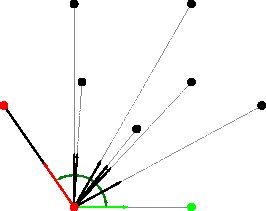
\includegraphics[width=0.5\textwidth]{giftW2d.pdf}~%
    %  \hbox to 0pt{\hspace*{-35mm}\raisebox{-110mm}[0pt][0pt]{а)}}

 \caption{Алгоритм Джарвиса. Определение следующей вершины}
 \label{fig:gw2}
\end{figure}


\subsubsection{Алгоритм Джарвиса на пространстве}\label{sec:gw3d}
Алгоритм является обобщением алгоритма заворачивание подарка на плоскости. Вместо прямой поворачивают плоскостью. Алгоритм описан в листинге \ref{alg:GWR3}.


\begin{algorithm*}[H]
    \caption{Алгоритм заворачивания подарка в $R^3$ - CH(P)}
    \label{alg:GWR3}
    \DontPrintSemicolon
    \KwIn{Множество точек $P$ \\$P=\{p_i|p_i=(x_1, x_2,\ldots, x_n)\in R^3, i=\left[1\ldots n\right]\}$ }
    \KwResult{Выпуклая оболочка множества точек $CH(P)$,\;заданная набором граней}
    Инициализировать пустой массив $C$\;
    Найти начальную грань $f_0$ выпуклой оболочки\;
    Добавить грань $f_0$ в $C$ \;
    Добавить грань $f_0$ в очередь $Q$\;
    \While{$Q \neq \varnothing$ \label{gift:whileStart}}
    {
        Выбрать и удалить грань $f$ из $Q$\;
        Добавить все ориентированные ребра $f$ в $A$\;
        \ForEach{ребра $e = p_i p_j \in A$}{
            Найти грань $f'$, состоящую из точек $\{p_j, p_i, p_l\}$\ и образующий максимальный угол с гранью $f$\;
            \If{$f'\notin C$ }{
                Добавить в в очередь $Q$ и массив $C$
            }
        }
    }
    \Return $C$
\end{algorithm*}

\subsubsection{Необщее положение точек}
При работе алгоритмов может возникнуть проблема необщего положения точек.
Если в гиперплоскости $R^n$ измерения лежит больше чем $n+1$ точка, возникает проблема построения грани в виде симплекса, в результате чего получается некорректно построенная выпуклая оболочка.

Метод Джарвиса на плоскости достаточно легко можно расширить для работы при необщем положении. Когда на прямой лежит больше чем 2 точки, берем самую дальнюю.

Но в трехмерном измерении и выше возникают более серьезные проблемы, не позволяющие корректно построить выпуклую оболочку.

% В случае работы алгоритма заворачивания подарка в трехмерном пространстве при необщем положении точек, может возникнуть случай, когда новонайденная грань лежит на уже найденной грани.


% Алгоритма заворачивания подарка на плоскости (см. раздел \ref{sec:gw3d}) в случае необщего положения точек. Алгоритм описан в разделе \ref{sec:gw3d}.
% Пусть $P = \{p_1, p_2, p_3, p_4, p_5\}$ - множество точек в $3$-мерном евклидово пространстве.
%В дипломной работе рассмотреть случай в 3d

\subsection{Постановка задачи работы}
Дано конечное множество точек $P=\{p_1,\ p_2,\,\ldots,\ p_m\}$ точек $p_i=(x_{1}^{i},\ x_{2}^{i}\ ,\ldots,\ x_{n}^{i})$ $R^n$-мерного евклидова пространства.

Точки могут находится в необщем положение, то есть в любой гиперплоскости $n$-мерного евклидова пространства может лежать больше чем $n+1$ точка.
Но основан на
В результате чего выпуклая оболочка может иметь несимплициальные грани.

Требуется построить выпуклую оболочку, т.е. найти наименьший выпуклый многомерный многогранник, содержащий все точки множества P.

\subsection{Реализация алгоритма}
В результате практической работы был разработан алгоритм построения выпуклой оболочки. (см. листинг \ref{alg:gift})
За основу алгоритма были взяты принципы работы алгоритма заворачивания подарка, поскольку он минимально использует специфику плоскости.

Рассмотрим работу алгоритма \ref{alg:gift}. В строке \ref{gift:ch2} происходит проверка, что точки являются двухмерными. Если это так, то вызывается метод построения выпуклой оболочки в двухмерном пространстве и алгоритм заканчивает работу. Алгоритм построения выпуклой оболочки на плоскости описан в разделе \ref{sec:ch2}.

В строке \ref{gift:firstFace} производится поиск начальной гиперграни. Алгоритм описан в листинге \ref{alg:firstFace}.

Далее просходит заполнение очереди $S$ гиперребрами начальной гиперграни.
Очередь $S$ хранит гиперребра, к которым еще не было найдено соседней гиперграни.

В множестве "H" (см. строку \ref{gift:initH}) хранятся список гиперребер, у которых уже были найдены соседние гиперграни. Это необходимо для заполнения очереди $S$ свободными гиперребрами из новонайденных гипергранней. Проверка и добавление гиперребер найденной гиперграни проиходит в строке \ref{gift:addedges}.

В строке \ref{gift:ifSimplex} проверяется, что являются ли найденные точки $P_g$ гиперплоскости симплексом. Если является, то вызывается отдельный метод построения симплицированной гиперграни.
Иначе происходит перенос точек $P_g$ в базис гиперплоскости и рекурсивный вызов метода для обработки множества точек $P_g$ .

% \subsection{Хранение выпуклой оболочки}

\begin{algorithm*}[H]
    \caption{Алгоритм построения выпуклой оболочки - $CH(P)$}
    \label{alg:gift}
    \DontPrintSemicolon
    \KwIn{Множество точек $P$ \\$P=\{p_i|p_i=(x_1, x_2,\ldots, x_n)\in R^n, i=\left[1 \ldots m\right]\}$ }
    \KwResult{Выпуклая оболочка множества точек $CH(P)$,\;заданная набором граней.
    }
    \If{$P\in R^2$ \label{gift:ch2}}
    {
        Найти выпуклую оболочку $CH_{2d}$ на плоскости при помощи метода Джарвиса\;
        \Return $CH_{2d}$\;
    }
    Инициализировать пустую выпуклую оболочку $CH$\;
    Инициализировать пустое множество использованных ребер $H$ \label{gift:initH}\;
    Найти исходную грань $F_0$ выпуклой оболочки\label{gift:firstFace}\;
    Добавить ребра $F_0$ в очередь $S$\;
    \While{$S \neq \varnothing$ \label{gift:whileStart}}
    {
        % $e=S.Pop()$\;
        Выбрать и удалить ребро $e$ из $S$\;
        Добавить $e$ в $H$\;
        %   $F=S.Pop()$\;
    %   \For{$e \in S$}
    %   {
        Найти гиперплоскость $g$, содержащую
        $CH ( e \cup p )$, где $ p \in P$, и все точки  $p_i \in P$ принадлежат нижнему полупространству плоскости $\pi$\;
        Найти множество точек $P_g = \{p_i|p_i\in P, p_i \in g, i=\left[1.. m_1\right]\}$ \label{gift:findFace}\;
        \If{$m_1 = n$ \label{gift:ifSimplex}}{
            Найти симплицированную грань $F$ \label{gift:chsimplex}
        }
        \Else{
            Найти координаты $P_g$ в базисе гиперплоскости $g$ \label{gift:crdbasis}\;
            $F$ = CH($P_g$)\;
        }
        \If{$P = P_g$ \label{gift:affin}}
        {
            \Return $F$\;
        }
        Добавить грань F в CH\;
        Добавить ребра $E=\{e_i |e_i \in F, e_i \notin H, i = \left[ 1\ldots m_2\right]\}$ в $S$\; \label{gift:addedges}
    %   }
    }
    \Return CH
\end{algorithm*}

\begin{algorithm*}[H]
    \caption{Алгоритм поиска первой грани - FindFirstFace(P)}
    \label{alg:firstFace}
    \DontPrintSemicolon
    \KwIn{Множество точек $P$ \\$P=\{p_i|p_i=(x_1, x_2,\ldots, x_n)\in R^n, i=\left[1\ldots m\right]\}$ }
    \KwResult{Выпуклая оболочка множества точек $CH(P)$,\;заданная набором граней
    }
    Инициализировать пустое множество точек $H$\;
    Найти минимальную точку $p_{min}$ множества $P$\;
    Добавить $p_{min}$ в $H$\;
    Найти плоскость $hp$ проходящую через точку $p_{min}$ с нормалью $\overline{n} = (1,0,0,\ldots,0,0)$\\
    \For{$n-1$ раз}{
        Поворотом плоскости вокруг вектора $\overline{n}$ найти гиперплоскость $hp_{next}$ проходящую через точки $H \cup p_{next}$, где $p_{next}\in P$ и дающая максимум скалярного произведения c плоскостью $hp$\;
        Добавить $p_{next}$ в $H$\;
        $hp$ = $hp_{next}$\;
    }
    Найти координаты точекы $H$ в базисе гиперплоскости $hp$ \label{firstPlane :crdbasis}\;
\Return CH($H$)
\end{algorithm*}
\newpage
\section*{Заключение}
\addcontentsline{toc}{section}{Заключение}
В данной работе был разработан алгоритм решение задачи построения выпуклой оболочки конечного набора точек $R^n$ размерности, находящихся в необщем положении.



Алгоритм не является окончательным и требует дальнейшей доработки.

Оставшиеся задачи и алгоритм будут доработаны в будущей выпускной работе.
\newpage

% Список литературы
\newpage
\addcontentsline{toc}{section}{Список литературы}
\begin{thebibliography}{}
	\bibitem{bib:preparata} Препарата Ф., Шеймос М. Вычислительная геометрия: Введение. под ред. Банковского Ю. М.~--- М.: Мир, 1989. --- 478~с.
    \bibitem{bib:Ivanov} Ивановский С. А., Преображенский А. С., Симончик С. К. Алгоритмы вычислительной геометрии. Выпуклые оболочки в трехмерном пространстве // КИО. 2007.
    \bibitem{bib:kokichi} Kokichi Sugihara,
    Robust gift wrapping for the three-dimensional convex hull //
    Journal of Computer and System Sciences,
    1994.
    391-407 c.,
\end{thebibliography}

\end{document}
